\documentclass[11pt]{article}

\usepackage{amsmath}                     % for some math formulas
\usepackage{enumerate}                   % for numearitions
\usepackage{amsthm}                      % for theorems
\usepackage{amssymb}                     % for some math symbols
\usepackage[matrix,arrow,curve]{xy}      % for diagramms \xymatrix{}
\usepackage{dsfont}                      % for operations like \mathbb{}
\usepackage{mathptmx}                    % LaTeX will use the Postscript Times type 1 font instead of the default ComputerModern font.
\usepackage{cancel}                      % for cross out the formulas
\usepackage{psfrag}
\usepackage{graphicx}
\begin{document}
\begin{figure}
\psfrag{a}{$\overrightarrow{a}$}
\psfrag{b}{$\overrightarrow{b}$}
\psfrag{bp}{$\overrightarrow{b}_{\parallel}$}
\psfrag{x}{$x$}
\psfrag{w}{$\omega$}
\psfrag{theta}{$\theta$}
\psfrag{y}{$y$}
\psfrag{O}{$O$}
\psfrag{v}{$\vec{v}$}
\psfrag{z}{$z$}
\psfrag{0}{$0$}
\psfrag{1}{$1$}
\psfrag{h}{$h$}
\psfrag{l}{$l$}
\psfrag{k1}{$k_1$}
\psfrag{k2}{$k_2$}
\psfrag{o}{$O$}
\psfrag{m}{$m$}
\psfrag{M}{$M$}
\psfrag{R}{$R$}
\psfrag{P}{$P$}
\psfrag{phi}{$\varphi$}
\psfrag{m}{$m$}
\psfrag{g}{$\overrightarrow{g}$}
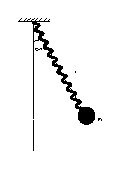
\includegraphics[width=4cm]{springPendulum.eps}
\end{figure}
\end{document} 